%=====================================================================
\section{Introduction}
\label{sec:intro}
Real-world networks are dynamic. Nodes and links appear and disappear, and interactions
such as face-to-face contacts, messages and citations occur at specific times. Classical
network analysis nevertheless aggregates these interactions into a single static graph in
which two nodes are either linked or not. Aggregation discards when links are active, how
often they recur, in which order they occur and how the network changes. Because
connectedness is not transitive in time, a temporal network cannot be reduced to a simple
graph without loss of information \citep{holme2015modern}, and the temporal-network
literature \citep{holme2012temporal,holme2015modern,masuda2016guide} has shown that each of
these features can alter conclusions about structure, communities and dynamical processes
such as epidemic spreading.

Most of this evidence derives from a single dataset or a single method, so the extent to
which temporal information matters, and for which kinds of system, remains unclear. This
study addresses that gap with two aims. The first is to quantify how temporal information
changes the characterization of the structure and function of real networks and how this
effect differs across network types (RQ1). The second is to determine in which systems the
hypotheses H1--H7 drawn from the literature (\cref{tab:hypotheses}) hold (RQ2).

\paragraph{Approach.}
The study is organised around four aspects of temporal networks (\cref{fig:framework}). The
first, representation, concerns the information lost by aggregation and by the choice of
time window. The second, activity patterns, concerns whether interactions are bursty,
repeated and persistent. The third, structural evolution, covers growth, ageing and the
reorganisation of communities, and the fourth, function, covers the effect of time ordering
on reachability, centrality and spreading. Each aspect is translated into hypotheses from
the literature, which are operationalised by metrics and tested against randomized
reference models \citep{gauvin2022randomized}. The resulting pipeline is applied to three
networks that differ in edge semantics, generating mechanism and temporal resolution: a
face-to-face contact network, an online messaging network and a citation network. Because
raw metrics are not comparable across such systems, the networks are compared through
hypothesis-specific time effects (\cref{sec:time-effect}).

\begin{figure*}[t]
\centering
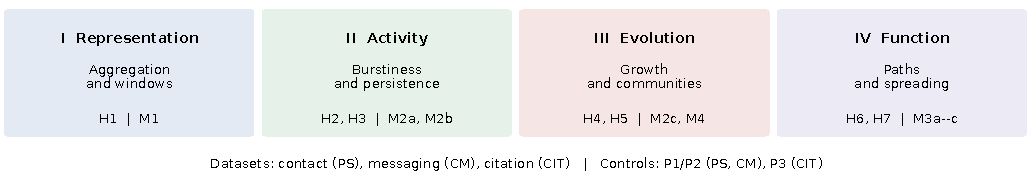
\includegraphics[width=\textwidth]{b_manuscript_framework.pdf}
\caption{Study design. Four aspects (Parts I--IV) map to seven hypotheses and four method
groups, in the order used throughout the paper. Reference models P1/P2 apply to PS and CM,
and P3 to CIT.}
\label{fig:framework}
\end{figure*}

\paragraph{Contributions.}
The study does not introduce new models. Its contribution is a question-driven synthesis of
the methods used to study temporal networks, a common and reproducible pipeline that applies
these methods to three types of empirical data, and a cross-network assessment of H1--H7
that identifies where temporal information is essential and where a static representation
suffices.

\paragraph{Organisation.}
\Cref{sec:related} reviews related work, \cref{sec:data} describes the data and
\cref{sec:methods} the methods. \Cref{sec:results} reports the results,
\cref{sec:discussion} discusses them and \cref{sec:conclusion} concludes.
